\section{The LLM whiteboard}

\begin{figure}[!h]
    \centering
    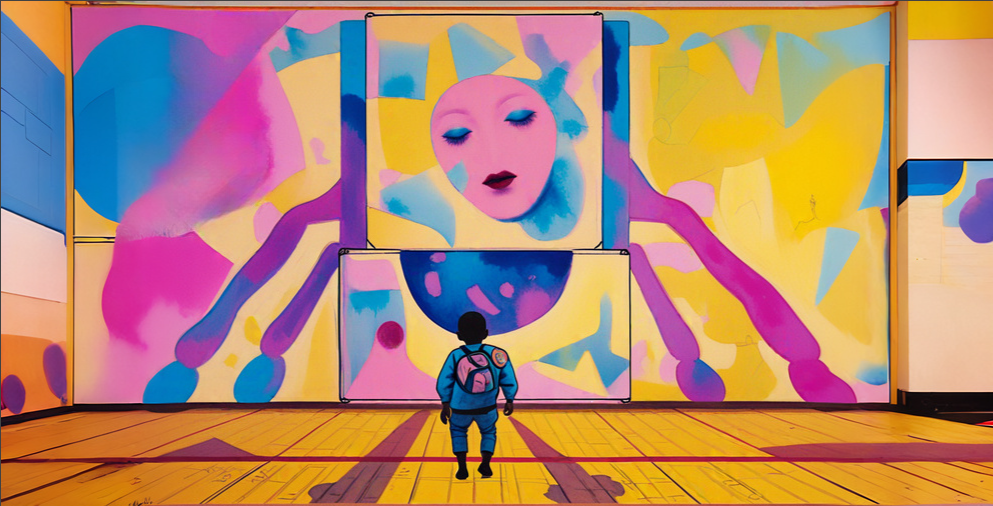
\includegraphics[width=\textwidth]{wBaordBanner.png}
    \caption{The spirit of the LLM WhiteBoard platform.}
    \vspace{0.1cm}
    \label{fig:spiritofWB}
\end{figure}

\subsection{ Introduction to the LLM Whiteboard}

\subsubsection{Objective and Scope}

The LLM Whiteboard is a collaborative platform that extends AI-driven interaction into both virtual and physical realms, empowering users to interactively code and create with minimal input and high flexibility.
Unlike tools designed to serve as “ghostwriters” such as GitHub Copilot\cite{chen2021evaluating}\cite{dakhel2023github}—the LLM Whiteboard goes beyond text-based code assistance, embracing an active role in creation by blending semantic operators with spatial interaction.
The project aims to redefine user affordances by allowing individuals to ideate and develop complex interactions without needing technical expertise, merging the simplicity of natural language commands with the depth of code-based design.

This project’s purpose is to explore AI-augmented affordances, focusing on real-time creation and adaptability in an environment that responds fluidly to high-level commands.
By positioning AI as an interpretive collaborator, the LLM Whiteboard enables an intuitive creative process that encourages both technical and non-technical users to engage with digital design through low-effort input and rich functionality.

\subsubsection{Key Concept Overview}

The LLM Whiteboard epitomizes the concept of low-signaling, high-possibility interfaces, where minimal signaling yields extensive creative potential.
By combining LLM-powered semantic interpretation with AR-enabled spatial interaction, the platform allows users to create and manipulate digital elements across two modes: an open canvas for purely digital, code-driven design and a AR environment that integrates digital creations into real-world contexts.
% This dual modality not only enhances the versatility of digital creation but also fosters a collaborative dynamic in which AI becomes an adaptive, responsive partner within an integrated digital and physical workspace.

\subsection{Collaborative Paradigms in AI and HCI}

\subsubsection{SpatialPixel and Collaborative Interaction}

Incorporating spatial affordances into digital interactions enhances both cognitive engagement and physical immersion, creating interfaces that better align with human cognition\cite{Kaptelinin2006ActingWT}.
Researchers Violet Whitney and William Martin, through their work at SpatialPixel, shown in figure \ref{fig:spatialpixel}, highlight the importance of spatial interaction in HCI.
Their work argues that cognition is deeply embodied and spatial, as human thoughts, actions, and problem-solving abilities are influenced by our physical surroundings.
Screen-based interfaces—often limited to flat layouts—can restrict this embodied cognition, confining digital interaction to a narrow scope that stifles creativity and collaboration.
Whitney and Martin term this limitation “flat screen, flat thoughts,”\cite{whitney2024} emphasizing the potential of spatial interfaces to support human cognition. 
% break free from these restrictions
SpatialPixel’s approach aligns digital interfaces with physical interactions, illustrating how we think through spatial organization, much as we do in physical workspaces\cite{andy1998extended}.
% Tools like Miro and Mural, which allow users to spatially arrange information, are early examples of how digital spaces can mimic physical work arrangements.
The concept of spatial cognition\cite{Nardi1995ContextAC}, which positions the surrounding space as integral to thought processes, thus serves as an essential framework for developing immersive, AI-enhanced interfaces that allow users to interact with systems in ways that feel intuitive and spatially grounded.

\begin{figure}[!h]
    \centering
    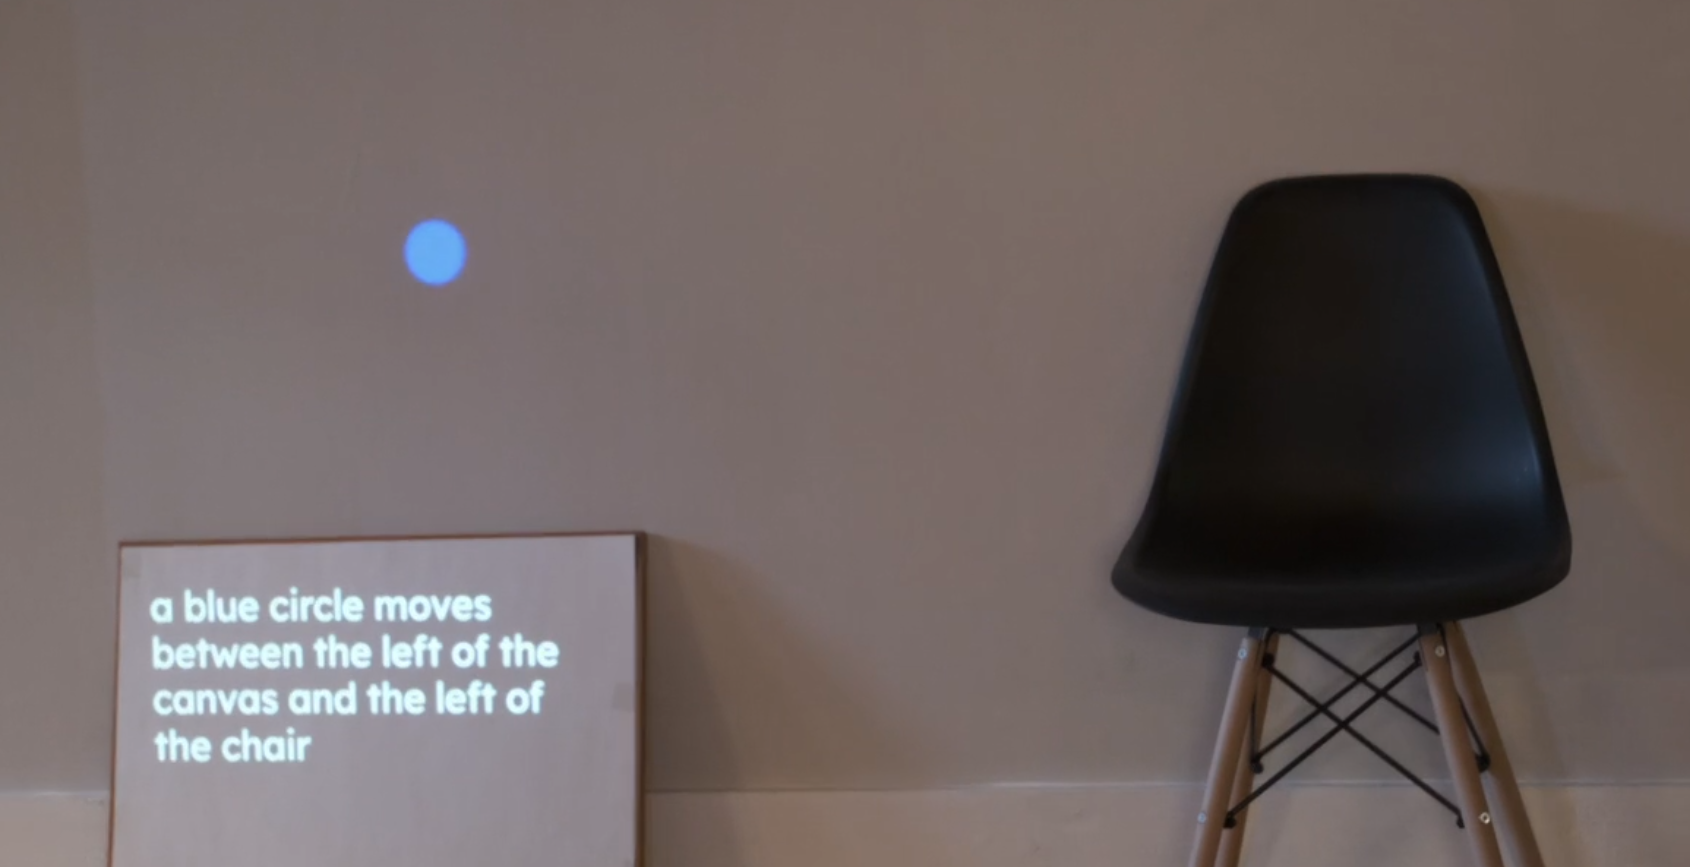
\includegraphics[width=\textwidth/3]{spatialpixel.png}
    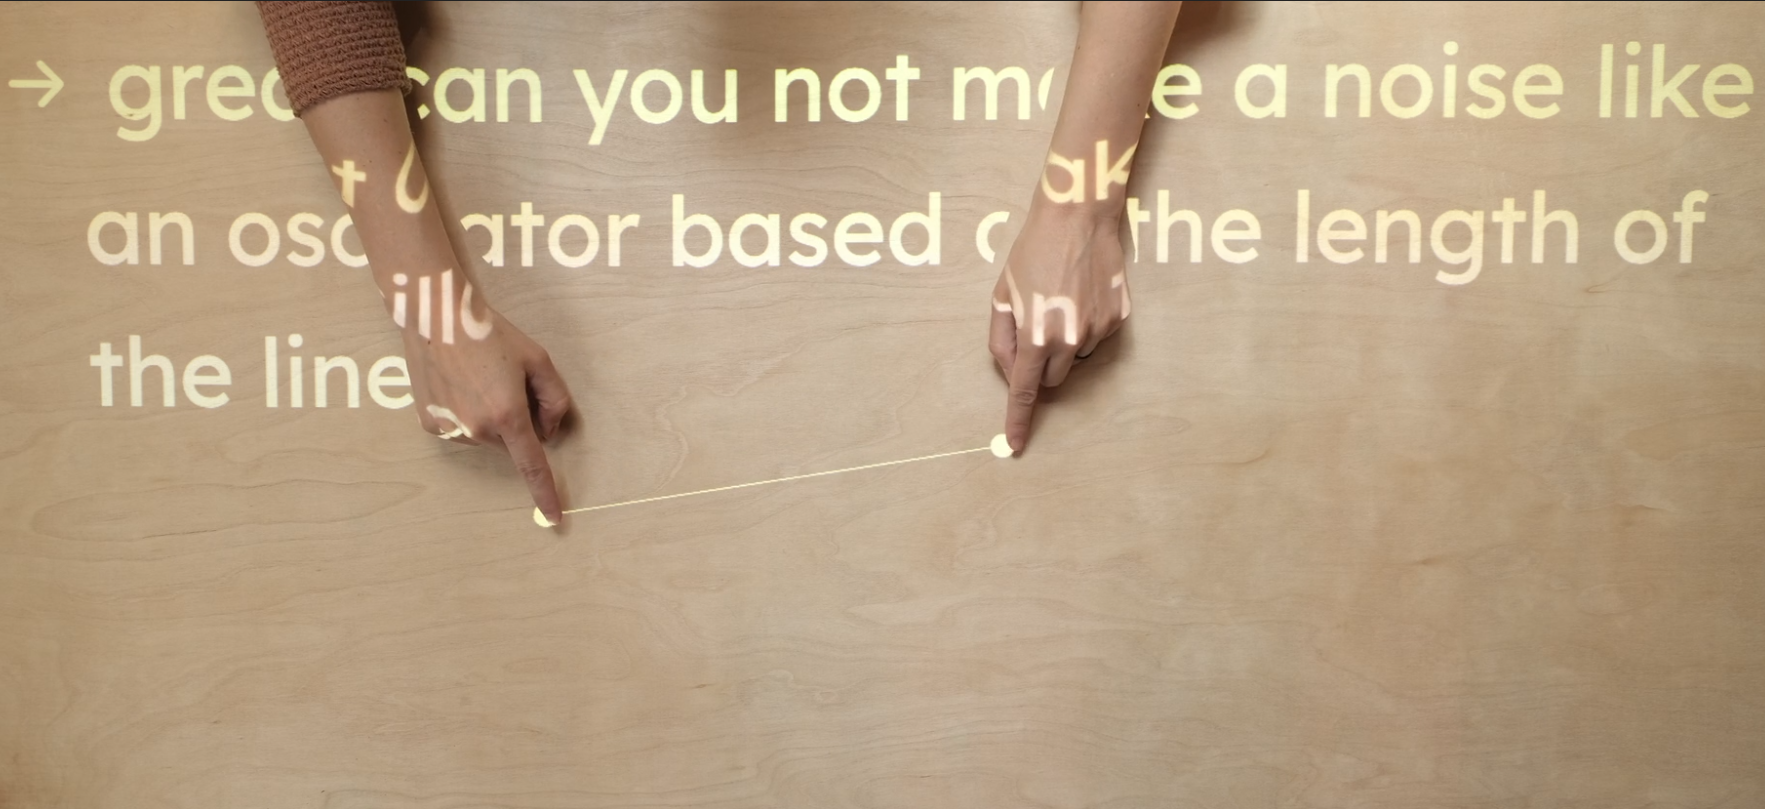
\includegraphics[width=\textwidth/3]{spatialpixel2.png}
    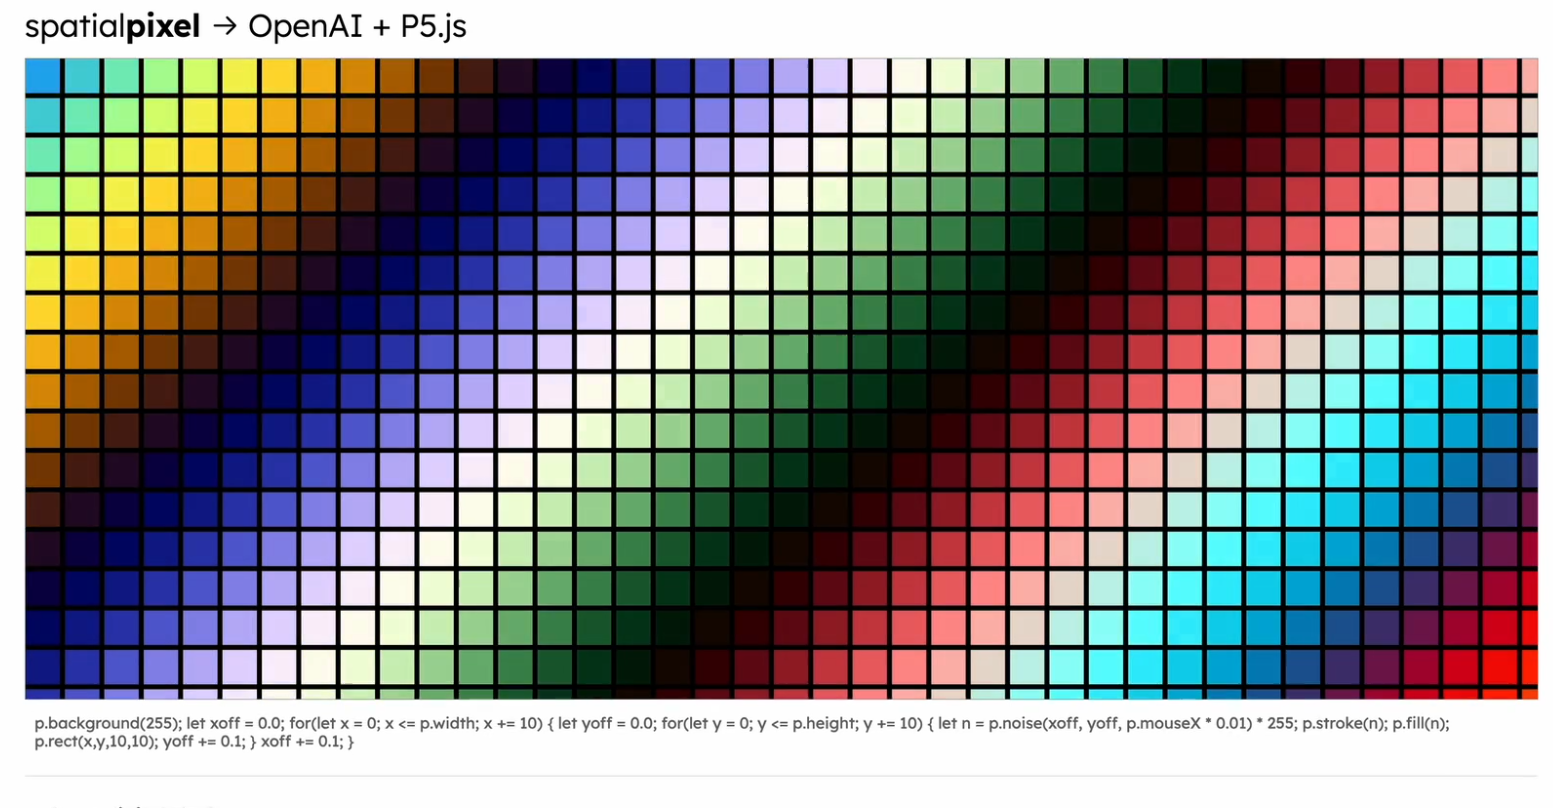
\includegraphics[width=\textwidth/3]{spatialpiwel3.png}
    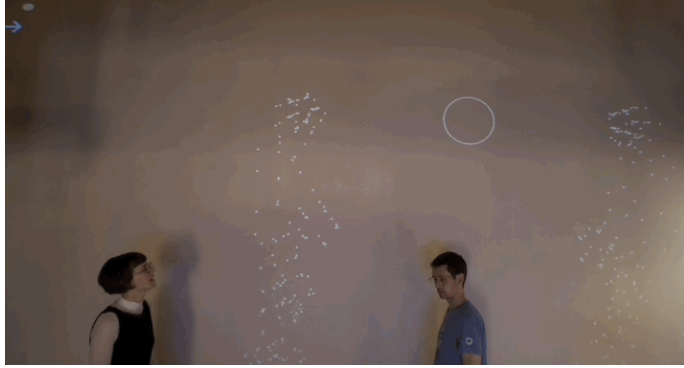
\includegraphics[width=\textwidth/3]{spatialPixel3.png}
    \caption{Showcase of SpatialPixel's work on integrating spatial paradigms in LLM assisted applications.}
    \vspace{0.1cm}
    \label{fig:spatialpixel}
\end{figure}

The LLM Whiteboard builds on SpatialPixel’s insights by combining the semantic understanding of LLMs with spatial affordances to enable more intuitive, embodied forms of collaboration.
Instead of merely generating code in response to commands, the LLM Whiteboard allows users to interact in a spatial context.
In AR mode, for example, users can physically engage with digital elements in real-world environments, bridging the gap between digital actions and physical gestures.
By enabling embodied interactions that extend beyond screen boundaries, the LLM Whiteboard enhances creative expression and aligns interaction with natural cognitive expectations.

\subsubsection{User-Centered Semantic and Spatial Interfaces}

A user-centered example demonstrates the fusion of semantic and spatial affordances in the LLM Whiteboard.
In AR mode, a user might point to a physical location, forcing the digital entities to update accordingly and creating an immersive exploration of the LLM generated code.
This interaction leverages the Mediapipe framework for spatial tracking, allowing the system to translate a simple physical gesture into a meaningful digital action.
Such an interaction not only aligns with human cognitive processes but also brings an intuitive physicality to digital creations, transforming how AI-enhanced environments are developed.

Through this combined approach, the LLM Whiteboard exemplifies a new HCI paradigm, where low-signaling input from the user generates high-possibility outputs.
Users can offload complex, technical commands onto the AI while retaining control over the creative and spatial arrangement of digital entities.
This intuitive balance between semantic and spatial interfaces creates a seamless creative workflow.

\subsection{From Semantic Operators to Semantic Algorithms}
\subsubsection{Reducing Complexity through Semantic Interpretation}
The LLM Whiteboard leverages large language models to interpret high-level user commands, transforming these into complex code without requiring users to engage with the underlying syntax or logic.
This shift resembles moving from a low-level programming language, like C, to a high-level language, such as Python.
However, in the case of the LLM Whiteboard, we achieve a more natural interaction by using the highest possible language—natural language—thus minimizing the cognitive load on users and simplifying interaction.

By translating broad user intents into precise code, the LLM reduces the technical barriers that often accompany creative digital work.
Users can specify what they want without needing to manage every technical detail, allowing the AI to handle these specifics.
This process exemplifies how LLMs serve as semantic operators, providing a fluid, intent-driven experience that broadens accessibility to digital content creation.

\subsubsection{LLM-Enabled Error Handling and Iterative Algorithms}

A unique feature of the LLM Whiteboard is its use of LLMs not just for code generation but for iterative code refinement.
The system writes, executes, and corrects code using error logs to refine outputs in alignment with user intent.
In this way, the LLM Whiteboard moves beyond single, linear prompts toward a more dynamic, iterative approach, improving its ability to respond to varied user needs and complex error cases.

When an error is thrown, the LLM analyzes the error log, cross-referencing it with both the user’s original command and the generated code to pinpoint and correct issues.
This iterative debugging process exemplifies how the LLM serves as a semantic algorithm, capable of aligning code output with user intent through cycles of self-correction.
By continuously refining the generated code based on real-time feedback, the LLM can adapt to a range of failure modes and error conditions, maintaining a responsive interaction loop.

\subsubsection{AI-driven Autonomy}
The LLM Whiteboard’s iterative approach draws inspiration from recent advancements in autonomous AI systems, such as BabyAGI\cite{nakajima2024} and AutoGPT\cite{autogpt2024}.
These projects highlight the value of iterative orchestration, where multiple rounds of refinement lead to more accurate and contextually relevant outputs.
In BabyAGI, for instance, recursive learning processes allow the model to learn from prior actions, progressively improving its responses to similar tasks.
Similarly, AutoGPT demonstrates how an LLM can break down high-level goals into sub-tasks, iterating on each to achieve more refined, autonomous task completion.

In the LLM Whiteboard, this iterative process is applied to real-time code execution and debugging.
As the LLM writes and tests code based on user commands, it actively refines outputs through self-assessment and correction, mirroring the recursive improvement seen in BabyAGI.
This model allows for a more dynamic interaction than traditional, single-prompt systems, empowering users to engage in complex creation workflows with minimal oversight or intervention.

\subsection{System Architecture and Core Technologies}

\subsubsection{ Langchain as a Semantic Orchestration Tool }
Langchain\cite{chase2022} serves as the primary orchestration framework in the LLM Whiteboard, managing real-time commands, interactions, and error correction to create a seamless user experience.
The logic used to achieve this is shown in figure \ref{fig:langchainlogic}.
Acting as an operational backbone, Langchain integrates the LLM with external tools and APIs, transforming it into a multi-functional system capable of handling diverse tasks dynamically.
This framework allows the LLM to interpret user commands and translate them into code, while also autonomously correcting errors and iterating over solutions.

\begin{figure}[h!]
    \centering
    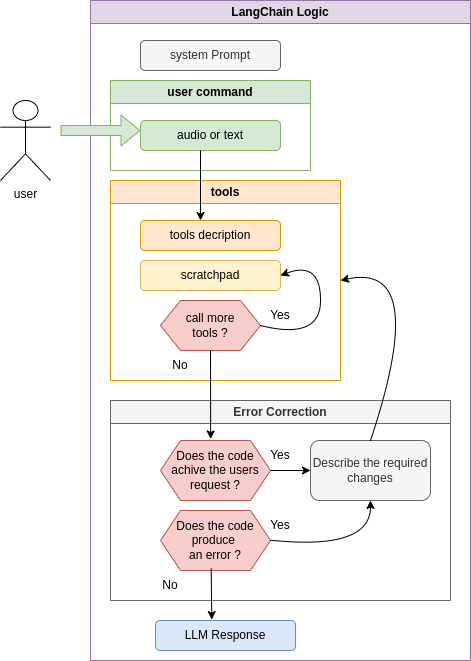
\includegraphics[width=\textwidth/2]{errorCL.drawio.png}
    \caption{Diagram of the LangChain Logic used for error correction.}
    \vspace{0.1cm}
    \label{fig:langchainlogic}
\end{figure}

Through zero-shot prompting, Langchain enables the LLM to generate new entities and functions on the fly by accessing predefined tools and APIs.
This structure allows for responsive, real-time engagement as Langchain dynamically adapts to the context of user inputs.
It also supports robust error correction, using fallback mechanisms that empower the LLM to autonomously refine its code, drawing on error logs to align outputs with user intent.
Langchain’s orchestration capabilities thus establish a foundation for creating adaptive, semantic-driven workflows that elevate the interactivity and fluidity of the Whiteboard.

\subsubsection{p5.js and Creative Coding}
p5.js provides the visual framework for real-time interaction within the LLM Whiteboard, transforming user commands into tangible graphical elements.
Known for its accessibility and playful approach to coding, p5.js offers an intuitive canvas that allows users to visualize and interact with their creations.
This ease of use makes it an ideal choice for lowering technical barriers, allowing users of all backgrounds to explore coding-based creation without needing advanced technical expertise.

Within the Whiteboard, p5.js enables the LLM to instantiate and manipulate entities—such as shapes, patterns, and animations—based on user instructions.
By offering instant visual feedback, p5.js supports an interactive coding environment that fosters experimentation and creativity.
Additionally, the LLM can extend p5.js’s core functionality, generating custom functions to further enhance the user’s creative possibilities.

\subsubsection{Mediapipe and AR Integration for Physical Interaction}
Mediapipe plays a central role in enabling the Whiteboard’s unique spatial interaction capabilities.
By capturing body movements and gestures and translating them into mathematical coordinates, Mediapipe enables LLM generated code to interface with a mathematical abstraction of the real world.
This integration aligns with the Whiteboard’s goal of combining semantic commands with spatial affordances.

In AR mode, Mediapipe detects physical gestures—such as pointing to a location or making a hand motion—allowing the LLM to generate corresponding digital elements in real-time.
This setup transforms the user’s physical presence into an interactive tool, enabling more natural and immersive forms of engagement.
Mediapipe thus supports a low-signaling, high-possibility interface, where users can interact with the digital world using minimal input while achieving complex outcomes.

\subsubsection{System Diagram}
The system architecture of the LLM Whiteboard maps out the interaction flow between user inputs, LLM processing, and visual outputs.
As shown in the architecture diagram on figure \ref{fig:wbarchietcure}, user inputs are fed into Langchain, which processes them through the LLM for code generation and error correction.
Commands are then directed to p5.js for visual rendering or to Mediapipe for spatial AR interactions.

\begin{figure}[h!]
    \centering
    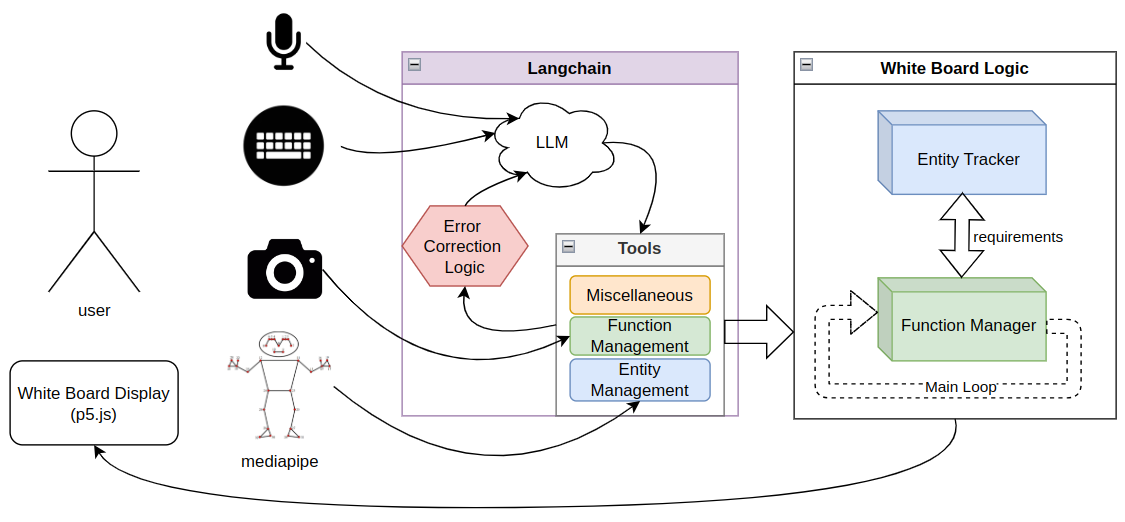
\includegraphics[width=\textwidth]{llmwhiteboard.drawio.png}
    \caption{Architecture diagram of the LLM WhiteBoard.}
    \vspace{0.1cm}
    \label{fig:wbarchietcure}
\end{figure}

The LLM Whiteboard provides multiple modalities for interaction, allowing users to engage via keyboard or voice commands.
This flexibility in command input further simplifies the user experience, while the integration of Mediapipe enables intuitive control over AR-based digital entities.
The Whiteboard also includes a drop-down menu, shown in figure \ref{fig:wbmenu}, where users can view and interact with the generated code, gaining a deeper understanding of the system’s functionality.

\begin{figure}[h!]
    \centering
    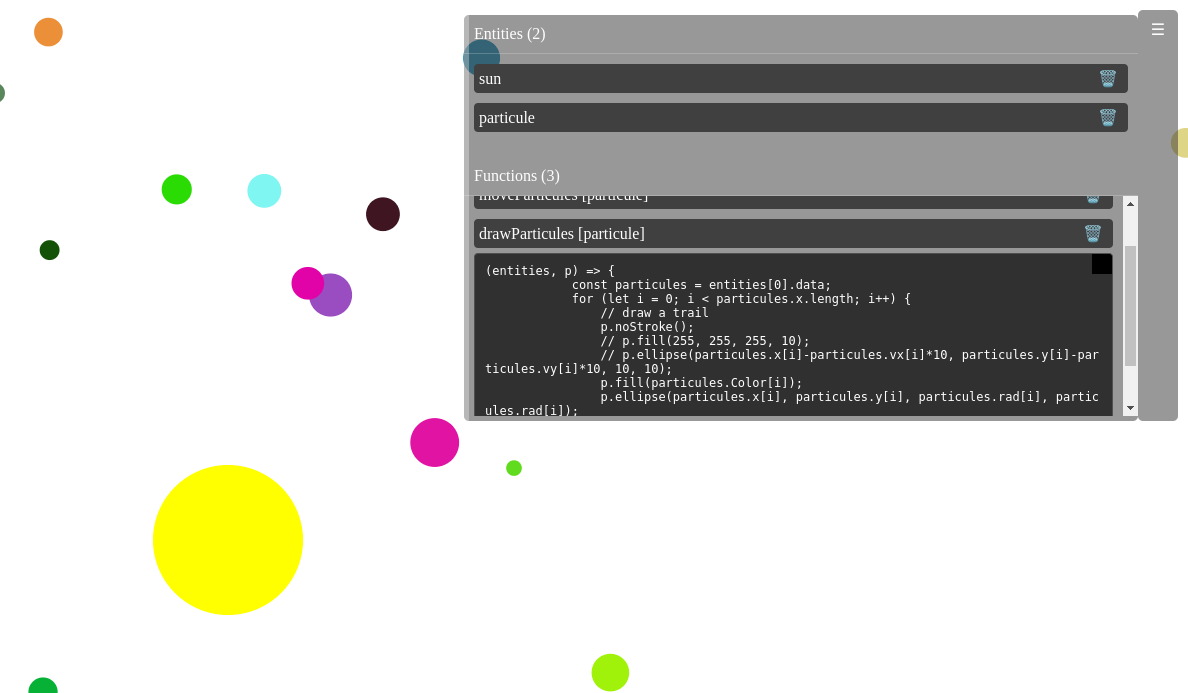
\includegraphics[width=\textwidth]{wbmenu.png}
    \caption{Menu allowing user to see the code generated by the LLM.}
    \vspace{0.1cm}
    \label{fig:wbmenu}
\end{figure}

Together, Langchain, p5.js, and Mediapipe form the core technologies at the foundation of the LLM Whiteboard, combining real-time semantic orchestration, dynamic visual feedback, and spatial interaction.
This integration enables users to explore a high-possibility, low-signaling interface that expands the potential for creative digital expression with minimal input and maximum expressiveness.

\subsubsection{Example of Command Execution }

The following is an example of a user asking the whitebaord to generate some animated circles:

\begin{enumerate}
    \item A user issues a command—either by typing or through voice-to-text—such as \emph{"draw a circle"}, the system parses the input and triggers the langchain pipeline.
    
    \item The command is fed to the LLM, which has access to a set of tools for managing both entities and functions.
    For the command \emph{draw a circle} the LLM selects to create a \textit{circle} entity and a \textit{drawCircle} function, representing its properties and its rendering process separately.
    
    \item Each tool is supported by a few-shot learning approach, which provides the LLM with examples of how similar commands were translated into code in the past.
    These examples follow a coding style based on an "arrays of objects" paradigm, designed to optimize performance as the number of entities and their properties scale.
    This separation into entities and functions helps keep graphical and logical components distinct, creating an organized and scalable structure for the generated code base.
    
    \item  The LLM-generated code is then executed within the live JavaScript environment.
    Any errors encountered during execution are logged and looped back to the LLM, enabling a refinement process that iteratively corrects and adapts the code.

    \item After each refinement, the code is re-evaluated to confirm that it meets the user’s objective.

    \item When the end of the generation cycle is reached, generated functions and entities are displayed on the p5.js canvas and in the management menu.

\end{enumerate}


% When a new command, such as \emph{"animate the circles"} is issued, the LLM leverages its existing understanding of the current environment, where it recognizes that a \textit{circle} entity already exists along with its corresponding \textit{drawCircle} function.
% The LLM thus focuses on generating only the necessary additions to fulfill the new command—in this case, a \textit{animateCircle} function.

The next user command might be \emph{"animate the circles"}.

\begin{enumerate}
    \item The LLM, equipped with memory of previous code and commands, identifies that the \textit{circle} entity and \textit{drawCircle} function already exist, meaning it only needs to add an animation function to the existing entity rather than recreating it from scratch.
    
    \item Using the tool for function creation, the LLM writes a \textit{animateCircle} function.
    This function may alter properties like position, size, or color over time, allowing the circles to move or change dynamically.
    
\end{enumerate}

Through this process, the LLM Whiteboard maintains a streamlined approach, reusing existing code structures and only introducing new functions as needed, creating a fluid and adaptive user experience.

\subsection{Modes of Interaction}

\subsubsection{White Board Mode}

% \textbf{Description and Interaction Flow}
In White Board mode, the LLM Whiteboard offers users an open canvas. % , where high-level commands transform into visual elements, facilitating creative exploration without the need for programming knowledge.
Users can type or speak commands like “create a circle” or “draw a wave pattern,” and Langchain orchestrates these inputs into corresponding p5.js code.%, enabling the LLM to interpret the commands and translate them into corresponding p5.js code.
Some of the possible outcomes are shown in figure \ref{fig:wbdemo1}.
This process abstracts the technical intricacies, letting users focus on their ideas while the system autonomously manages the code generation.

\begin{figure}[h!]
    \centering
    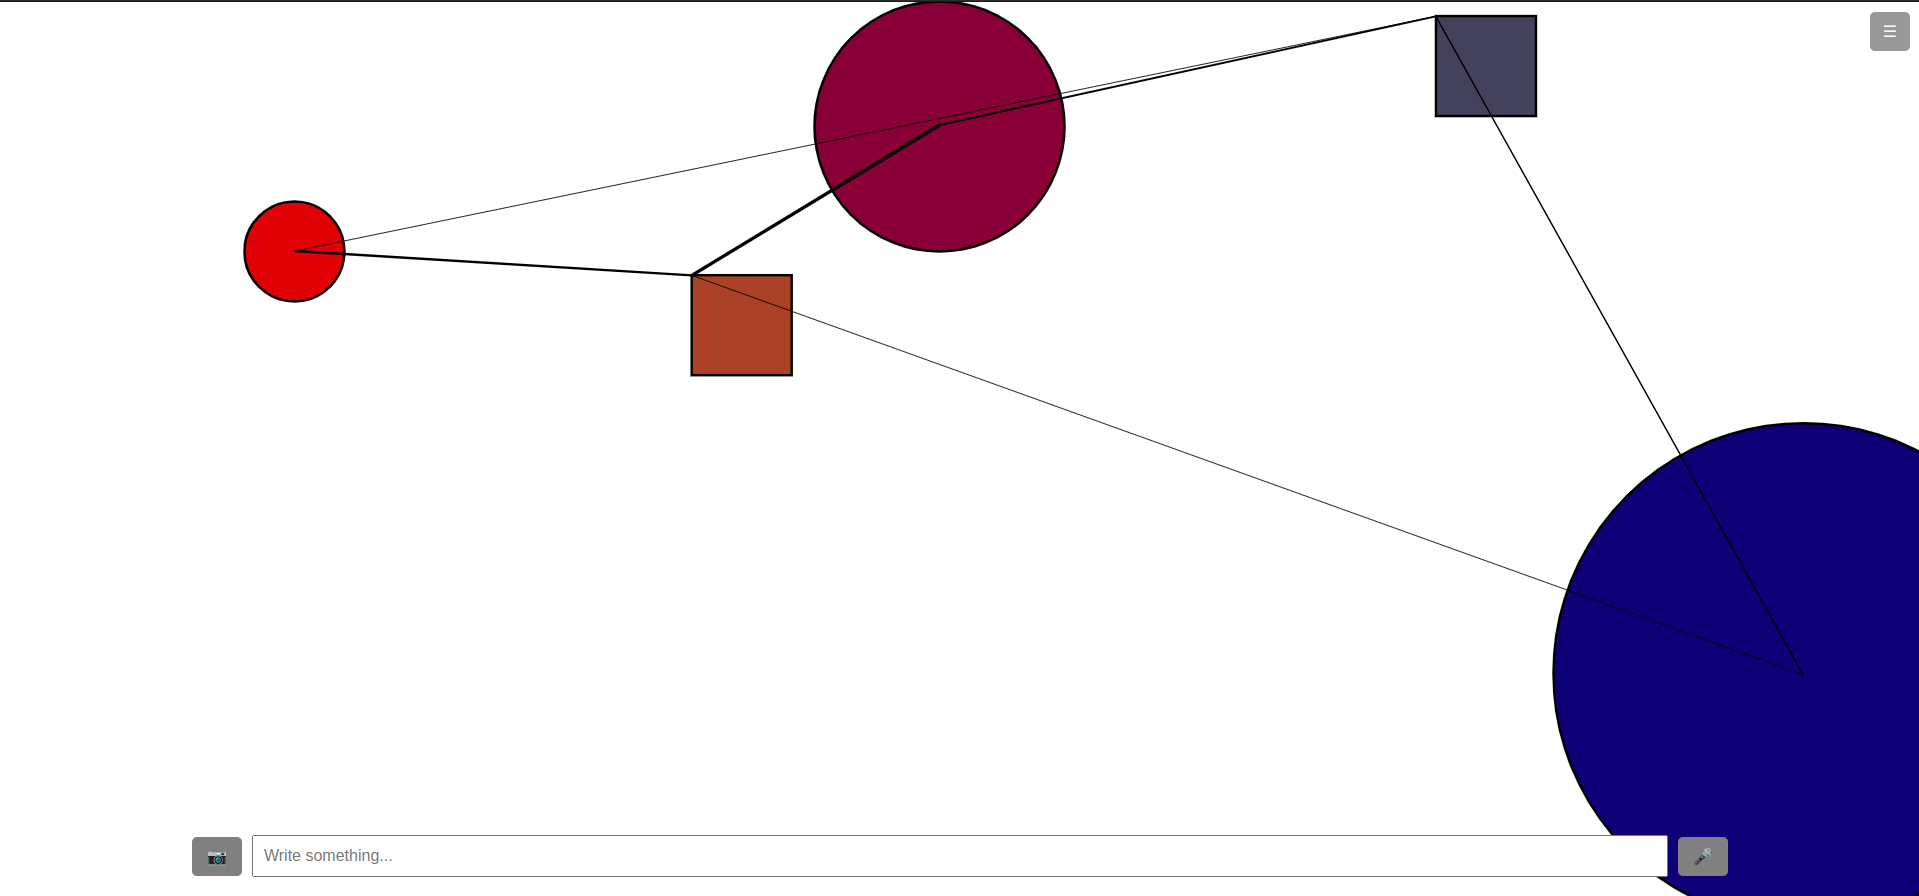
\includegraphics[width=\textwidth/2]{wbexp1.png}
    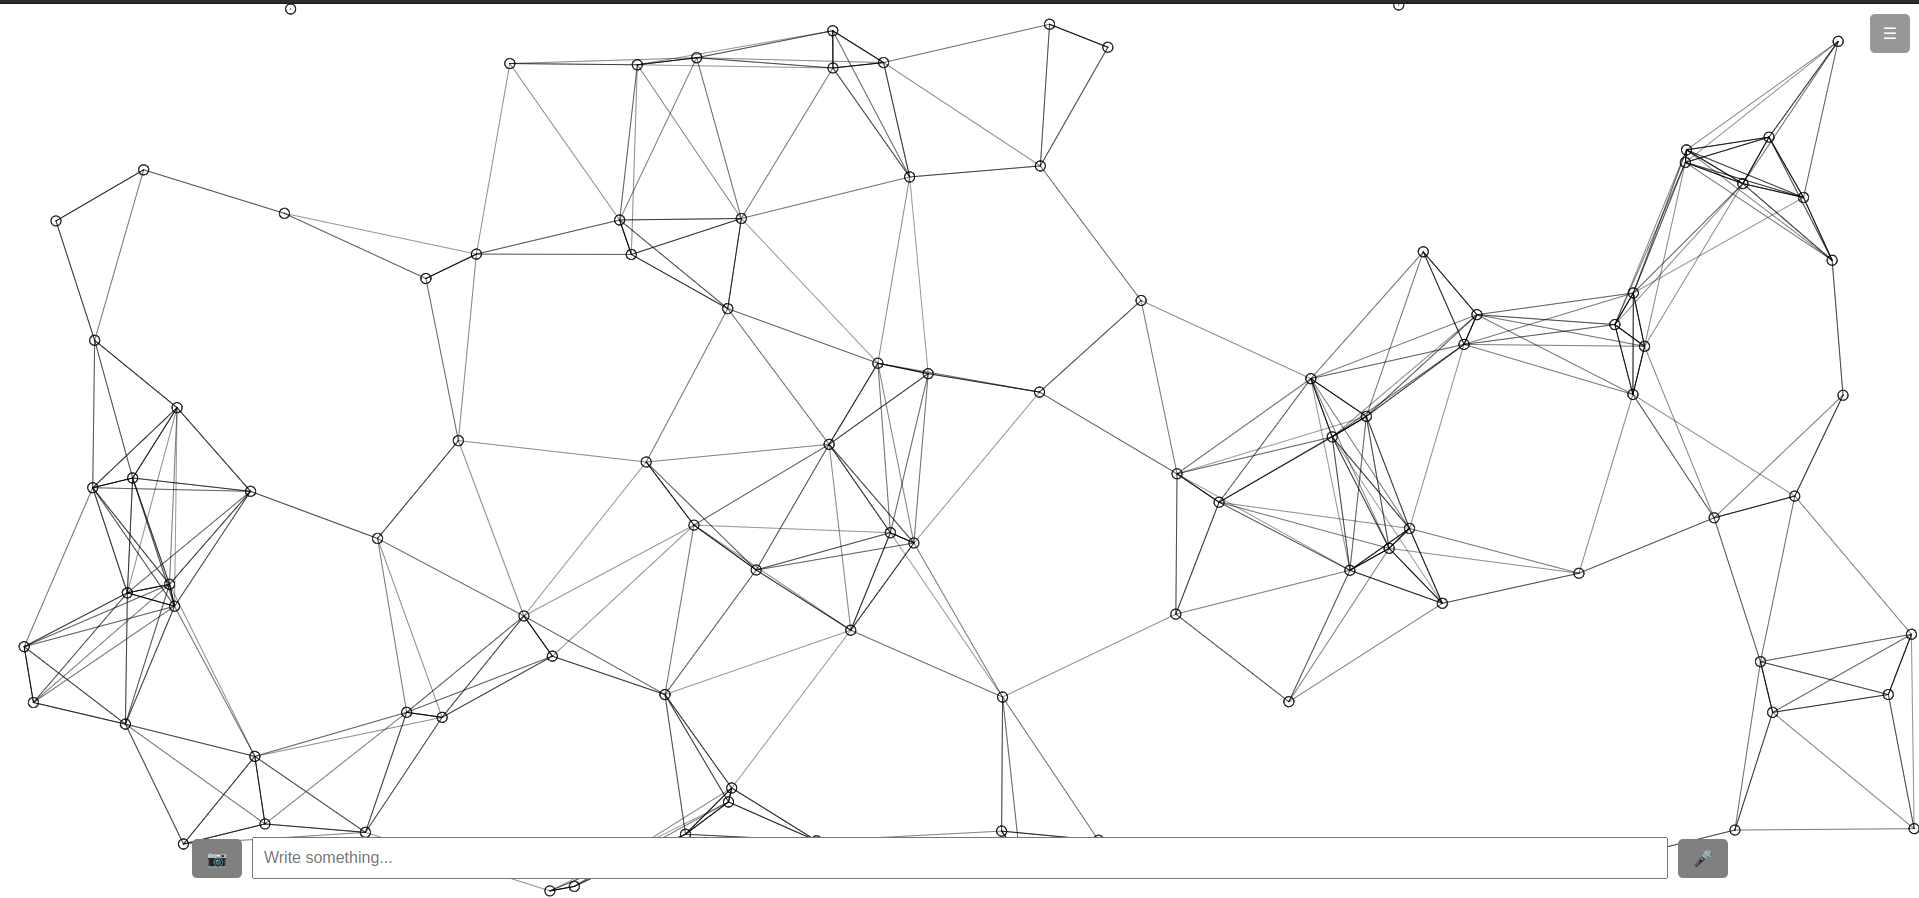
\includegraphics[width=\textwidth/2]{wbexp2.png}
    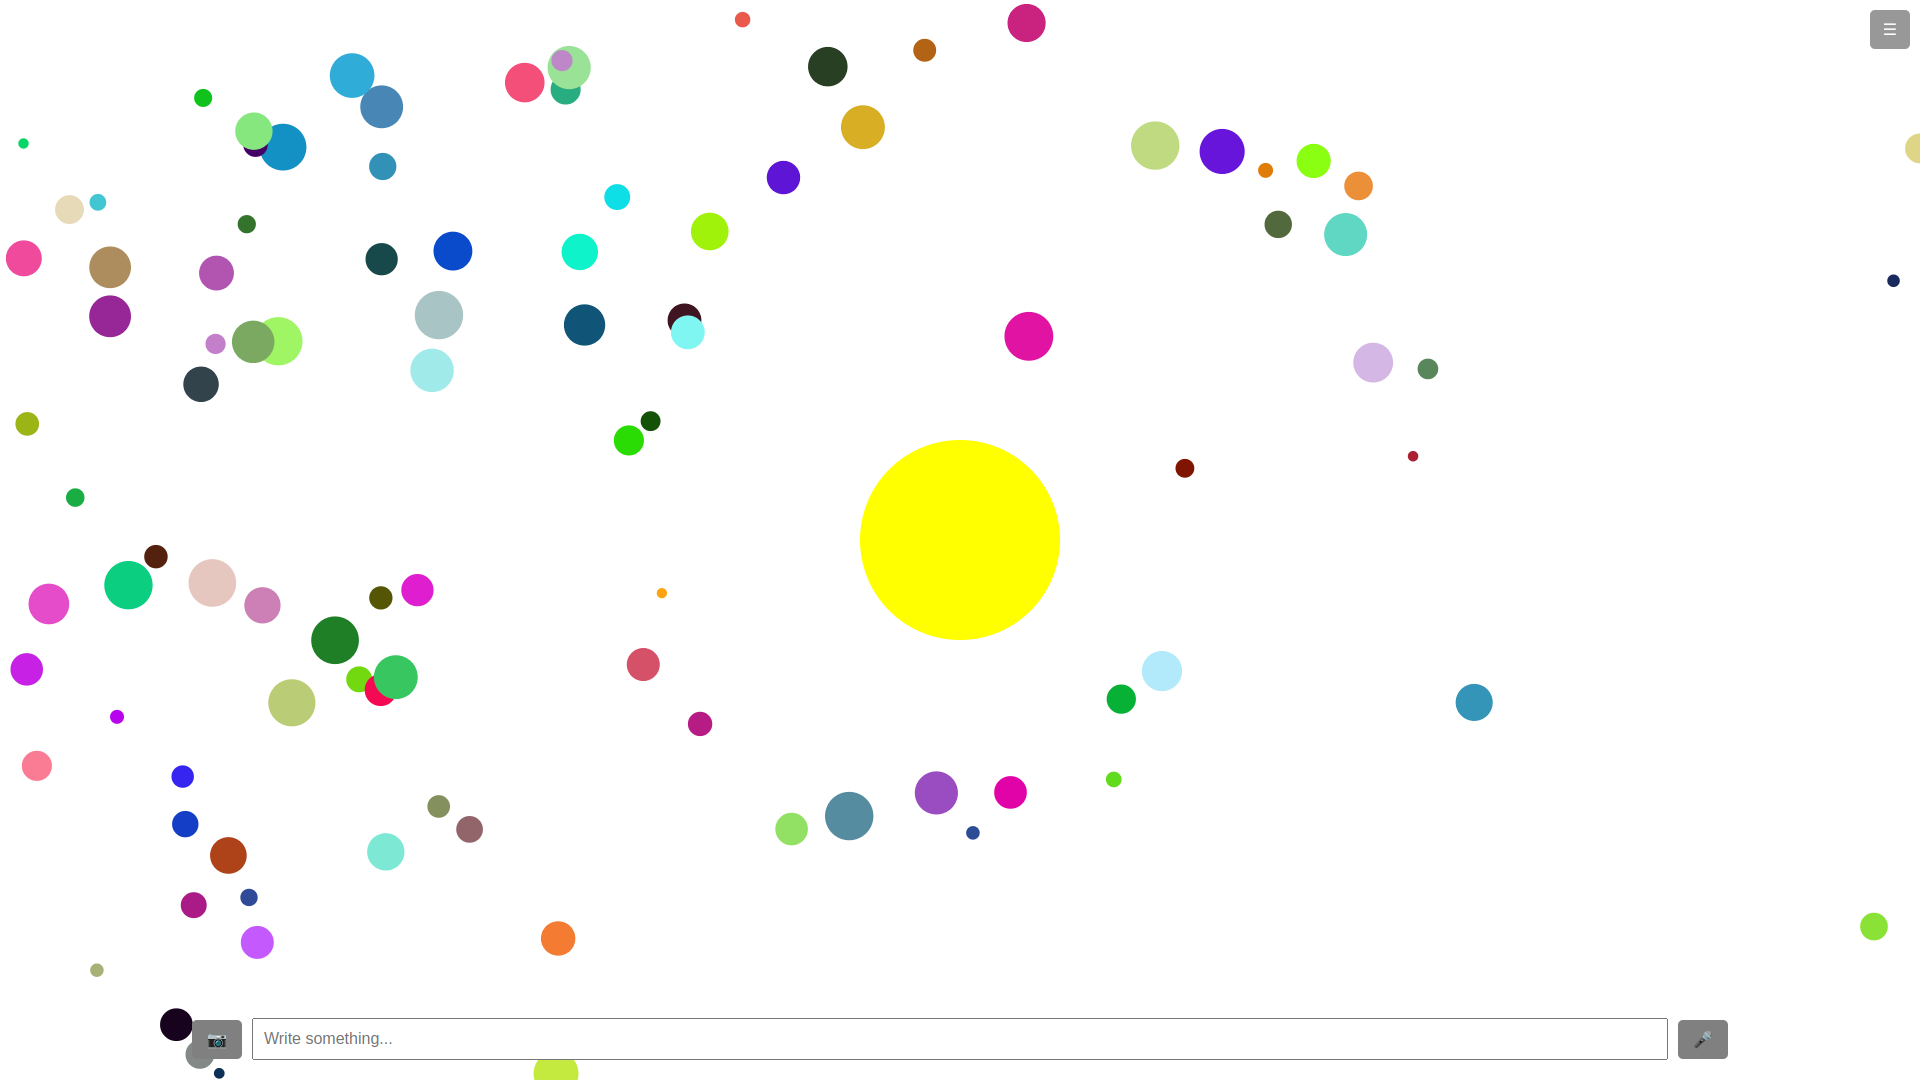
\includegraphics[width=\textwidth/2]{wbexp3.png}
    \caption{Demonstration of the LLM WhiteBoard in action.}
    \vspace{0.1cm}
    \label{fig:wbdemo1}
\end{figure}

The interaction flow is fluid and iterative: users input commands, and the LLM generates visual feedback on the canvas.
% This real-time response empowers users to interact dynamically with their creations, adjusting inputs as needed to achieve desired outcomes. ithout the need for programming knowledge
This real-time response empowers users to interact dynamically with their creations.% without the need for programming knowledge
By decoupling user input from coding syntax, the White Board mode makes creative coding accessible and engaging for users across different skill levels.

% \textbf{Error Correction and Iterative Creation}
To ensure a seamless user experience, Langchain manages error correction through iterative refinement.
% When the generated code encounters an issue, Langchain analyzes error logs and cross-references the error with the user’s command and initial code.
% The LLM then iteratively corrects its output, addressing issues on the fly.
This capability allows users to create continuously without interruptions from code errors, providing a smooth creative process.
% The iterative error correction mechanism is a key feature of White Board mode, enhancing reliability and user satisfaction by aligning outputs with user intent through minimal interaction.

% \textbf{User Affordances}
The White Board mode exemplifies a low-signaling, high-possibility interface, where users provide simple, abstract commands that yield complex, meaningful outputs.
This approach empowers users to explore intricate designs with minimal effort, allowing them to build complex visual compositions through a straightforward interaction model.
The system’s affordances thus lower technical barriers, inviting users to delve into creative coding without requiring detailed knowledge of syntax or programming logic.

\subsubsection{AR Mode (Spatial Interaction)}

% \textbf{Real-World Overlay and User Engagement}
AR mode in the LLM Whiteboard introduces an immersive experience by overlaying digital content onto the user’s real-world environment.
This mode leverages Mediapipe for real-time tracking of body movements, enabling physical interaction with digital elements.
As users move or gesture, their actions directly influence the digital space, blending the physical and virtual realms to create a mixed-reality environment.
This real-world overlay allows users to manipulate virtual objects with their gestures, making spatial interaction a central part of the creative process.

% \textbf{Example Interactions}
% In AR mode, user commands are translated into actions that respond to physical gestures.
For instance, a user could command, “make the circles follow my hands,” and then use hand motions to position the circles within the AR space.
Other commands might involve actions like changing an object’s color with a hand gesture or resizing elements by moving closer or farther from the camera.
A sample of possibilities are shown in figure \ref{fig:wbdemo2}.

\begin{figure}[h!]
    \centering
    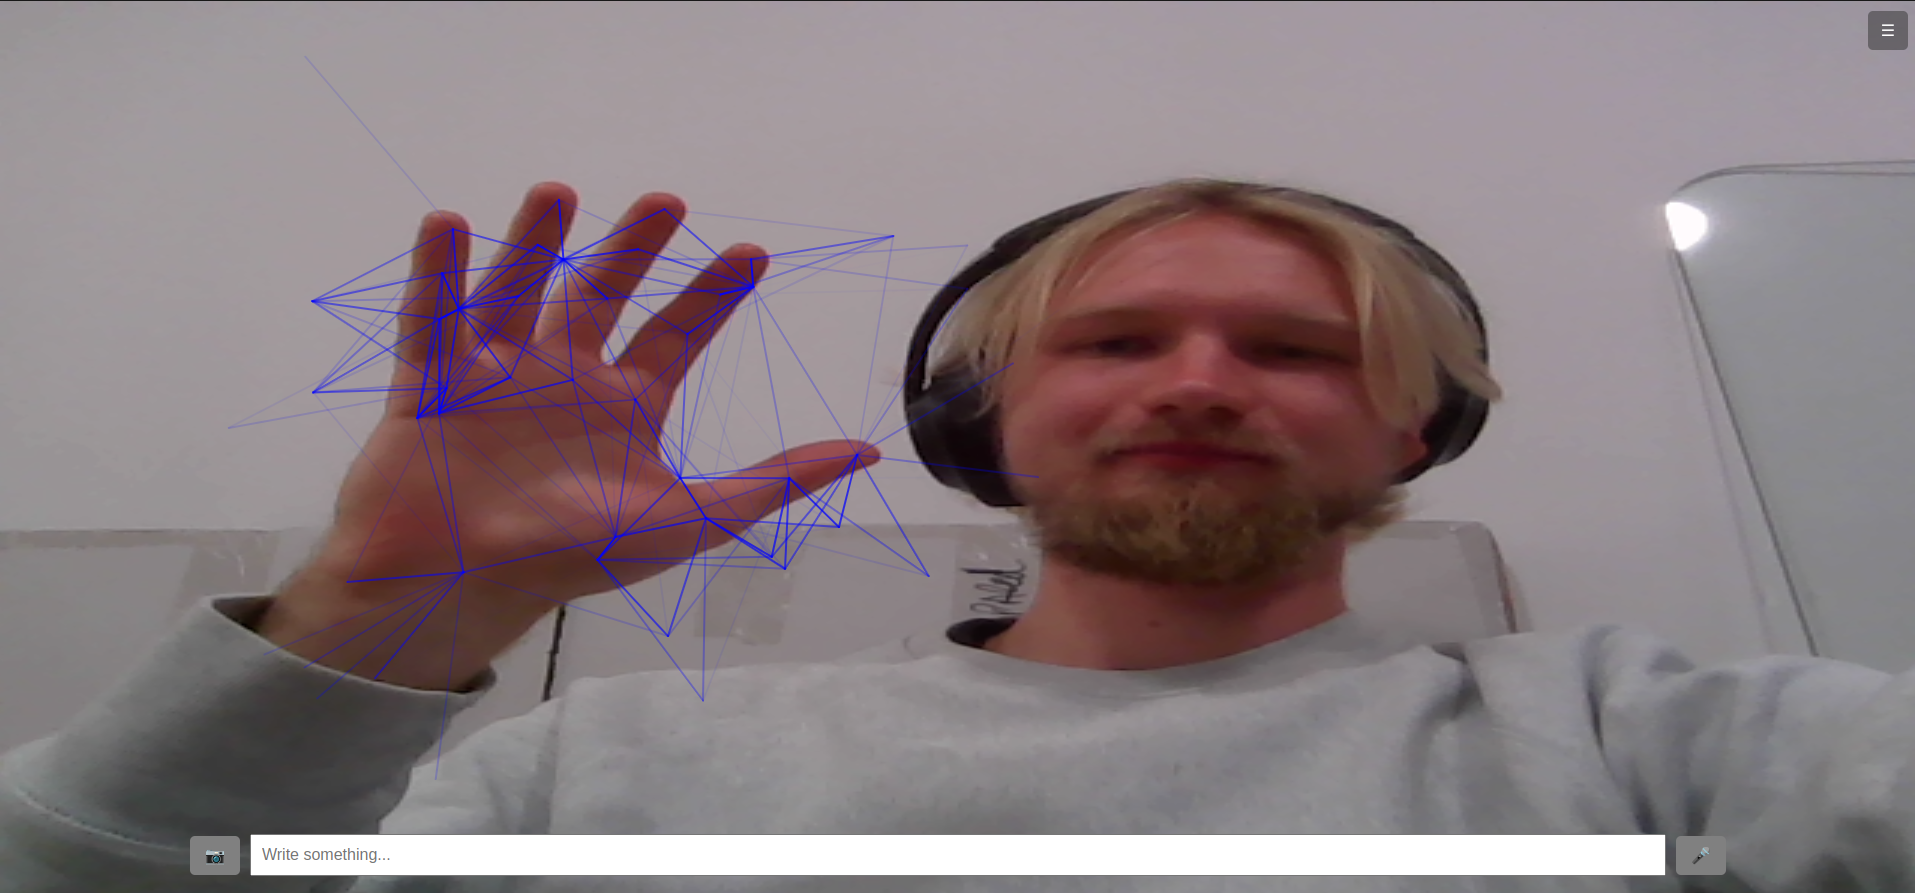
\includegraphics[width=\textwidth/2]{wbexpar1.png}
    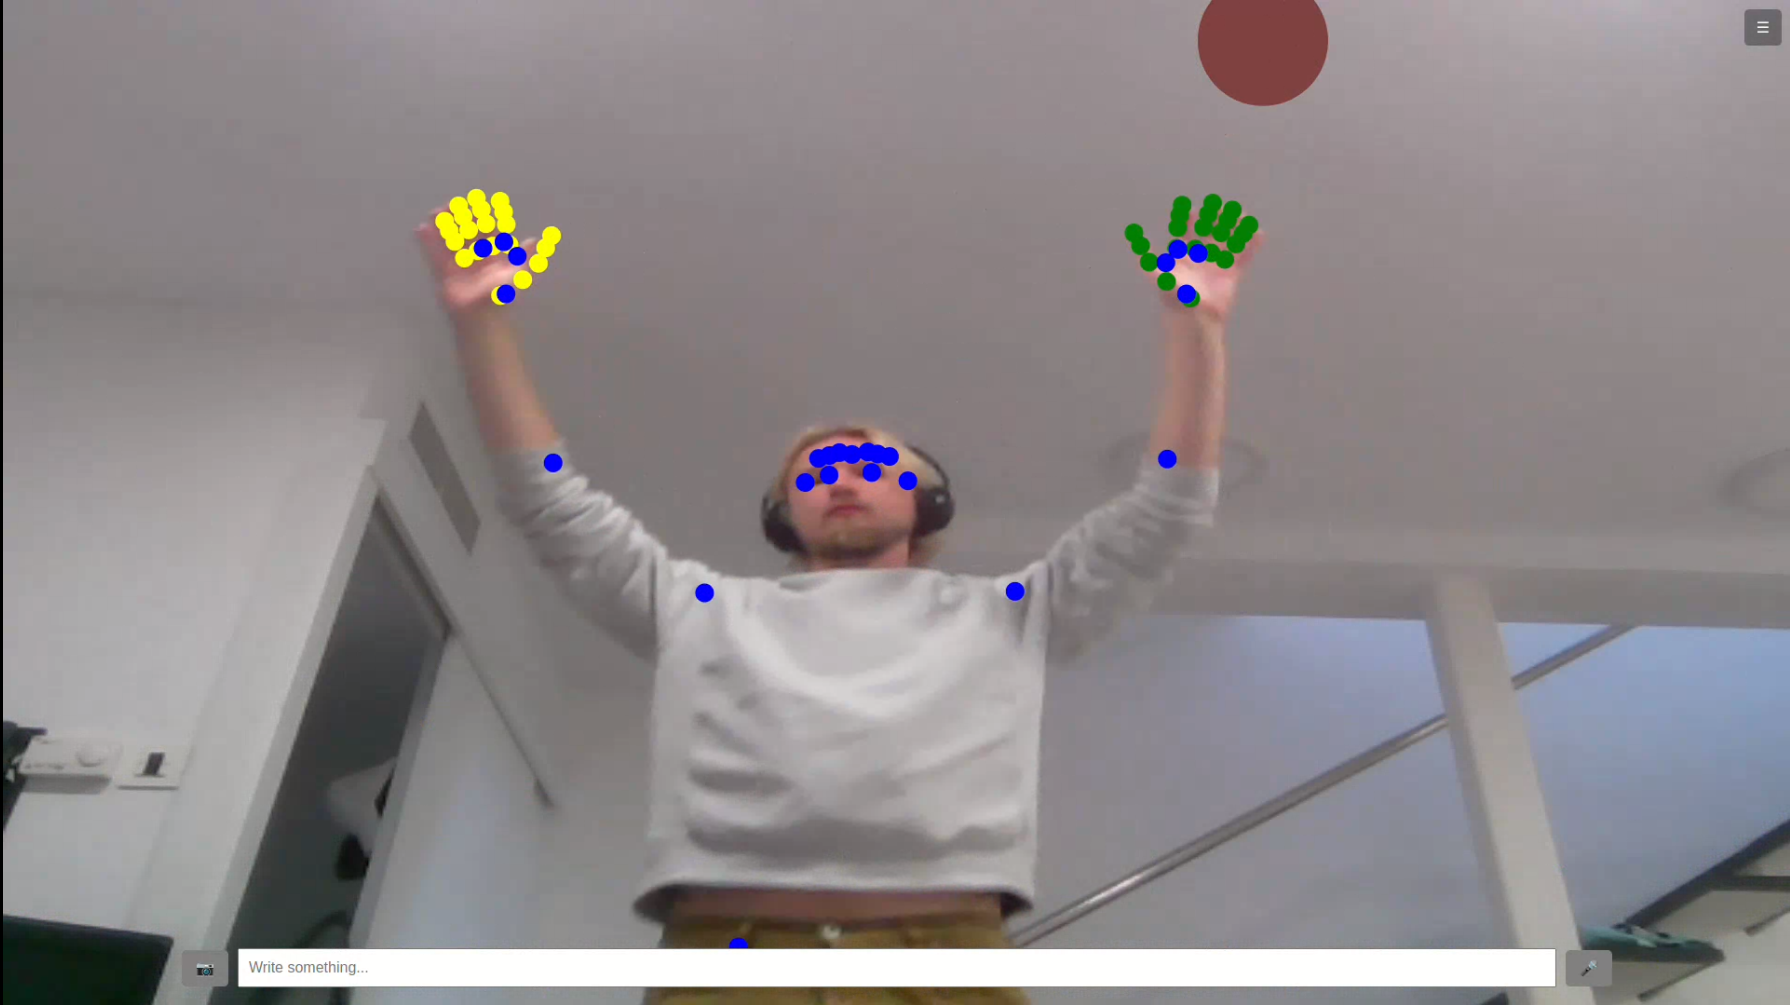
\includegraphics[width=\textwidth/2]{wbexpar2.png}
    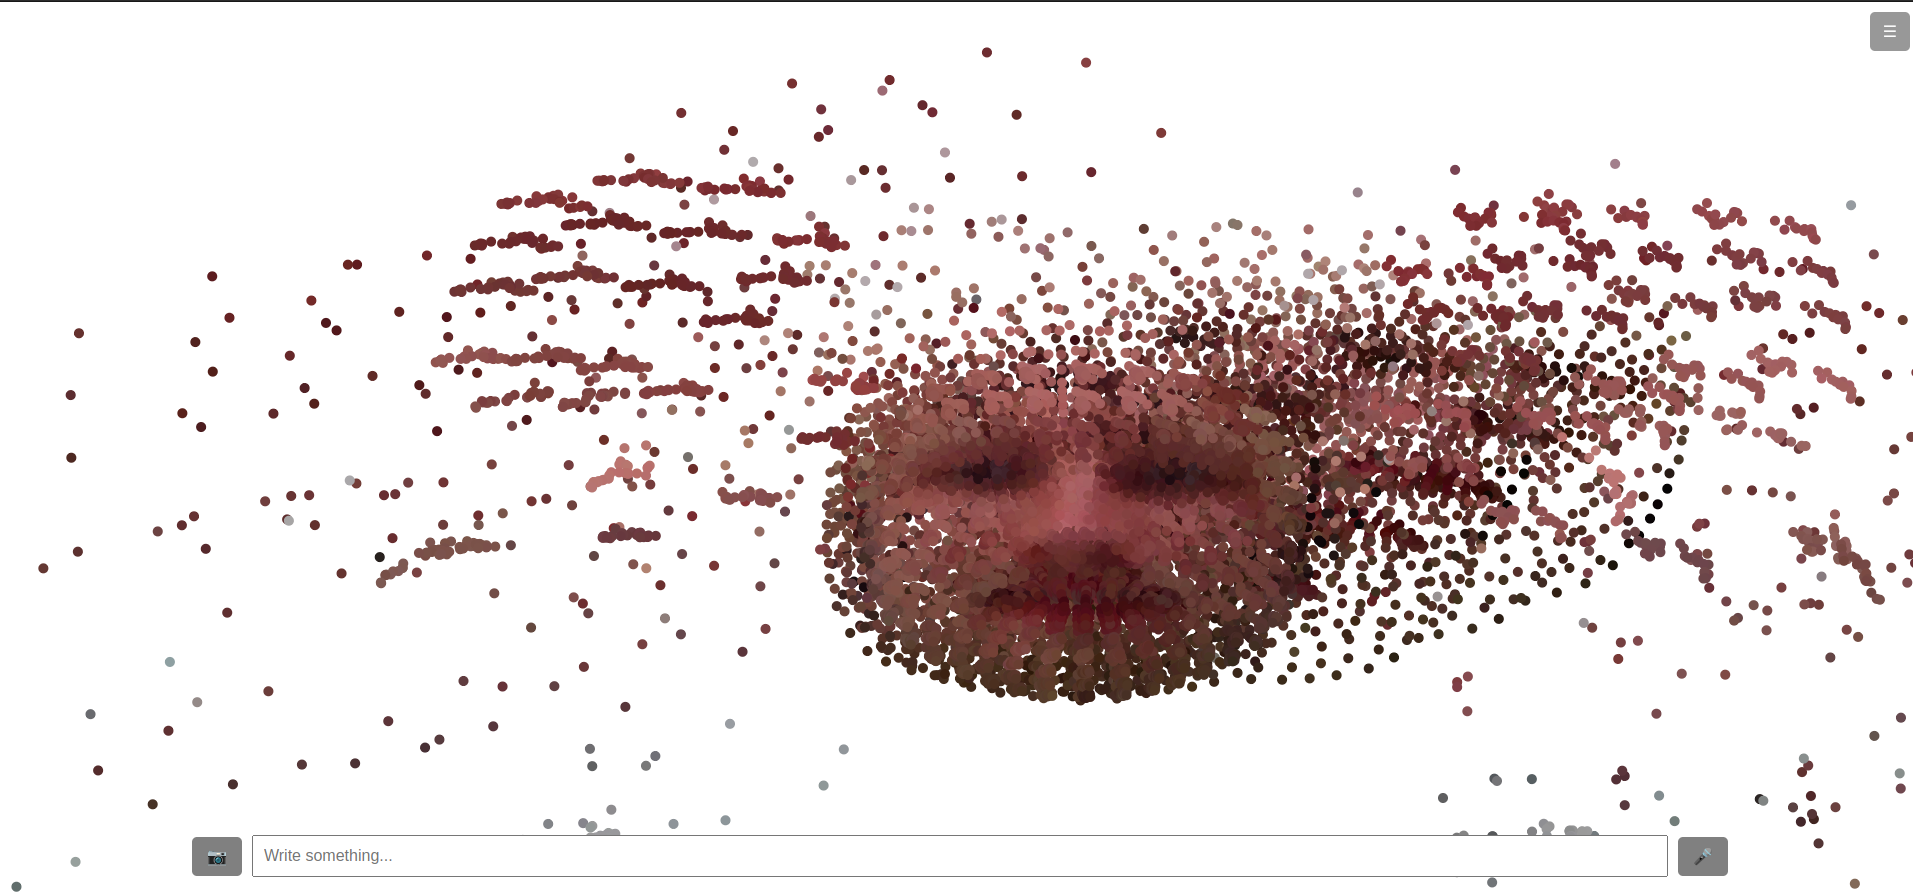
\includegraphics[width=\textwidth/2]{wbexpar3.png}
    \caption{Demonstration of the AR mode of the LLM WhiteBoard in action.}
    \vspace{0.1cm}
    \label{fig:wbdemo2}
\end{figure}

These interactions illustrate how users’ natural movements extend into the digital environment, creating an intuitive interface that fosters a responsive and immersive experience.

% \textbf{Embodied Cognition and Immersion}
By capturing the user's body movements and interpreting them as interactive commands, AR mode aligns with principles of embodied cognition, which suggest that physical actions shape cognitive processes.
The immersive environment created by the LLM Whiteboard allows users to think and interact spatially, leveraging natural gestures to control digital entities.
This embodied approach to interaction not only enhances creative potential but also strengthens the connection between the user and the digital space, offering an engaging, collaborative experience.
Users can move freely within their physical surroundings while manipulating digital elements, opening new avenues for immersive digital expression and real-time spatial interaction.


\subsection{Project Review and Insights }

The LLM Whiteboard demonstrates how the integration of semantic language models with AR-based spatial interaction can reshape HCI, turning high-level commands into dynamic, interactive creations.
The platform’s dual modes—White Board mode for open, visual coding and AR mode for immersive spatial engagement—enable users to move beyond traditional coding constraints.
By reducing the complexity of digital creation, the Whiteboard provides both technical and non-technical users with an accessible, intuitive interface that combines creative coding and spatial interaction.

The Whiteboard’s design exemplifies low-signaling, high-possibility affordances, where minimal input from users yields sophisticated outcomes, making it a powerful tool for exploring new AI-driven collaborative models in HCI.

\subsubsection{Discussion}

The Whiteboard repositions AI as more than a tool, framing it as a creative collaborator capable of transforming user intent into functional code.
This dynamic challenges traditional views on AI’s role in creative processes, inviting users to engage in a co-creative relationship with AI.
As AI systems like the Whiteboard take on a more collaborative role, they also prompt important questions about creative control, artistic ownership, and the evolving boundary between human and machine-driven creativity.

The AR mode leverages spatial interaction to foster a more engaging, intuitive experience aligned with embodied cognition.
By connecting physical gestures with digital responses, the Whiteboard enables users to engage with digital elements naturally, effectively extending cognitive processes into the digital space.
This spatial engagement aligns with theories such as Extended Mind Theory\cite{andy1998extended}, where cognition is distributed beyond the brain and body, into the surrounding environment through interactive tools.
Through spatial affordances, the Whiteboard enriches the user’s problem-solving and creative potential, providing an immersive, hands-on approach to digital creation.

A significant contribution of the Whiteboard lies in its accessibility.
By abstracting away coding complexities, it enables a wider range of users to participate in digital design and interaction, fostering inclusivity within HCI.
This democratization of technology aligns with broader trends in HCI that seek to make advanced tools accessible to all.
In making interactive digital creation more approachable, the Whiteboard demonstrates how AI-augmented platforms can expand access to creativity and innovation.

\subsubsection{Final Thoughts}
% The LLM Whiteboard sets a compelling precedent for the future of HCI by integrating AI’s semantic power with spatial interaction, providing a glimpse into the potential of AI-driven, user-centered design.
% The project opens pathways for future exploration where AI and AR combine to create immersive, adaptive environments that transcend traditional interface boundaries, promoting creativity and enhancing user agency.

% By merging AI-driven autonomy with spatial interactivity, the Whiteboard lays the groundwork for HCI applications that prioritize human-centric, collaborative digital experiences.
% The implications for HCI are vast, signaling a future where AI enhances human capabilities within digital spaces, offering tools that feel as intuitive and responsive as they are powerful and transformative.

The LLM Whiteboard sets a compelling precedent for the future of HCI by integrating AI’s semantic power with spatial interaction, providing a glimpse into the potential of AI-driven, user-centered design.
This project demonstrates how language models can interpret and respond to high-level commands, enabling users to intuitively generate complex outcomes with minimal input.%, which marks a significant step toward more accessible and responsive interfaces.
Beyond individual user interactions, the LLM Whiteboard opens pathways for future exploration where AI and AR combine to create immersive, adaptive environments that transcend traditional interface boundaries, promoting creativity and enhancing user agency.

By merging real-time spatial cues with dynamic language processing, this platform can evolve to support multi-user, collaborative experiences that adapt based on context.
This convergence of AI-driven affordances and spatial engagement sets the stage for environments that do not merely respond to user actions but anticipate needs and offer relevant, context-aware support.
Future iterations of such systems could extend beyond creative coding, finding applications in education, therapy, and collaborative workspaces where AI-augmented interfaces serve as powerful partners.